\chapter{PHÂN TÍCH VÀ MÔ HÌNH HÓA}
 
% ============================================================
\section{Mô phỏng chuyển động robot bằng phần mềm MATLAB}
% ============================================================
 
\subsection{Tính toán động học}
 
\subsubsection{Hệ tọa độ và phép đổi hệ}
 
Chương trình sử dụng ba hệ tọa độ:
\begin{itemize}
    \item \textbf{Hệ body}: gắn với thân robot, dùng để khai báo vị trí khớp hông (hip) và điểm đặt chân trung tính.
    \item \textbf{Hệ world}: dùng để biểu diễn robot trong không gian 3D toàn cục.
    \item \textbf{Hệ local}: gắn với từng chân, dùng để giải động học của từng chân bằng một bộ công thức chung.
\end{itemize}
 
Việc chuẩn hóa cả 6 chân về cùng một hệ quy chiếu cho phép dùng chung một hàm động học nghịch và động học thuận cho toàn bộ robot, giúp đơn giản hóa đáng kể quá trình lập trình.
 
\begin{figure}[H]
    \centering
    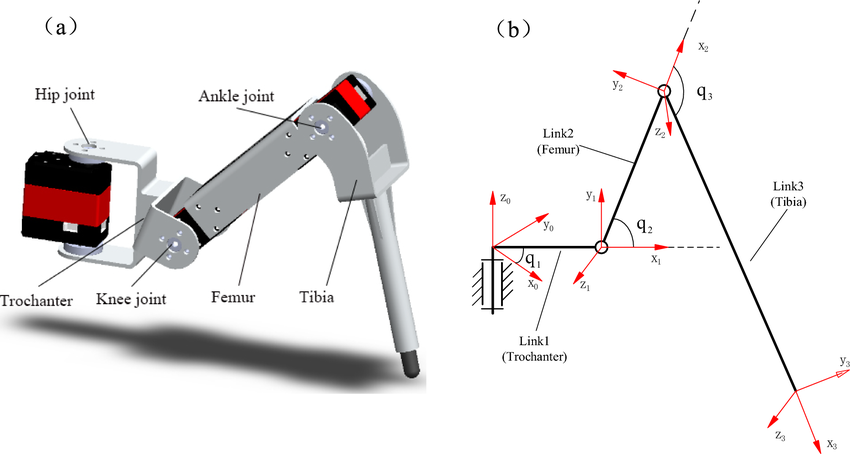
\includegraphics[width=0.85\textwidth]{pictures/coordinate_system.png}
    \caption{Sơ đồ hệ tọa độ và phép đổi hệ giữa các chân robot}
    \label{fig:coord_system}
\end{figure}
 
\subsubsection{Động học thuận và động học nghịch}

\hspace{0.5cm} Mỗi chân robot có 3 bậc tự do với các khớp Coxa ($q_1$), Femur ($q_2$), Tibia ($q_3$) và chiều dài đoạn tương ứng $L_1$, $L_2$, $L_3$.

\textbf{Động học thuận (Forward Kinematics):} Cho trước góc khớp $(q_1, q_2, q_3)$, tính tọa độ bàn chân trong hệ local của chân:

\begin{equation}
    p = L_1 + L_2 \cos q_2 + L_3 \cos(q_2 + q_3)
\end{equation}
\begin{equation}
    X = p \cos q_1, \qquad Y = p \sin q_1
\end{equation}
\begin{equation}
    Z = L_2 \sin q_2 + L_3 \sin(q_2 + q_3)
\end{equation}

trong đó $p$ là tầm với nằm ngang từ gốc khớp Coxa đến bàn chân.

\textbf{Động học nghịch (Inverse Kinematics):} Cho trước vị trí bàn chân $(X, Y, Z)$ trong hệ local, tính ngược lại các góc khớp:

\textbf{Bước 1} — Góc Coxa:
\begin{equation}
    q_1 = \mathrm{atan2}(Y,\, X)
\end{equation}

\textbf{Bước 2} — Khoảng cách nằm ngang từ gốc Femur đến bàn chân và đường chéo tổng hợp:
\begin{equation}
    d = \sqrt{X^2 + Y^2} - L_1, \qquad D = \sqrt{d^2 + Z^2}
\end{equation}

Điều kiện tồn tại nghiệm: $|L_2 - L_3| \leq D \leq L_2 + L_3$.

\textbf{Bước 3} — Góc Tibia (định lý cosin):
\begin{equation}
    \cos q_3 = \frac{D^2 - L_2^2 - L_3^2}{2\,L_2 L_3}, \qquad q_3 = \arccos(\cos q_3)
\end{equation}

\textbf{Bước 4} — Góc Femur:
\begin{equation}
    q_2 = \mathrm{atan2}(Z,\, d) - \mathrm{atan2}\!\left(L_3 \sin q_3,\; L_2 + L_3 \cos q_3\right)
\end{equation}

Cấu hình elbow-down (dấu $+$ trong $q_3$) được chọn để đảm bảo khoảng tĩnh không dưới thân robot.


\subsubsection{Phép đổi hệ tọa độ body sang local}

\hspace{0.5cm} Mỗi chân $i$ được gắn vào thân robot tại một góc định hướng $\psi_i$ đo từ trục $X$ thân (ngược chiều kim đồng hồ). Các giá trị $\psi_i$ của 6 chân lần lượt là: LF $45°$, LM $90°$, LB $135°$, RF $-45°$, RM $-90°$, RB $-135°$.

Khi bàn chân có tọa độ $(X_b, Y_b, Z_b)$ trong hệ body, tọa độ tương ứng trong hệ local của chân $i$ được tính bằng phép quay ngược chiều góc $\psi_i$ quanh trục $Z$:

\begin{equation}
    \begin{bmatrix} X_l \\ Y_l \end{bmatrix}
    =
    \begin{bmatrix} \cos\psi_i & \sin\psi_i \\ -\sin\psi_i & \cos\psi_i \end{bmatrix}
    \begin{bmatrix} X_b \\ Y_b \end{bmatrix},
    \qquad Z_l = Z_b
\end{equation}

Trong chương trình MATLAB, phép đổi hệ này được áp dụng cho cả hip lẫn bàn chân trước khi giải IK, đảm bảo bộ công thức IK chung được dùng cho tất cả 6 chân mà không cần viết riêng cho từng chân.


\subsubsection{Tính lại động học thuận để dựng lại chân}

\hspace{0.5cm} Sau khi có $(q_1, q_2, q_3)$ từ IK, động học thuận được áp dụng để tính lại bốn điểm mốc của chân trong hệ local, phục vụ vẽ cấu trúc xương chân lên đồ thị:

\begin{itemize}
    \item $P_0$: gốc khớp Coxa (hip) — điểm gốc hệ local, $(0,\, 0,\, 0)$.
    \item $P_1$: điểm cuối đoạn Coxa:
        \begin{equation}
            P_1 = P_0 + L_1\,\begin{bmatrix}\cos q_1 \\ \sin q_1 \\ 0\end{bmatrix}
        \end{equation}
    \item $P_2$: điểm cuối đoạn Femur:
        \begin{equation}
            P_2 = P_1 + L_2\,\begin{bmatrix}\cos q_1 \cos q_2 \\ \sin q_1 \cos q_2 \\ \sin q_2\end{bmatrix}
        \end{equation}
    \item $P_3$: điểm cuối đoạn Tibia (bàn chân):
        \begin{equation}
            P_3 = P_2 + L_3\,\begin{bmatrix}\cos q_1 \cos(q_2+q_3) \\ \sin q_1 \cos(q_2+q_3) \\ \sin(q_2+q_3)\end{bmatrix}
        \end{equation}
\end{itemize}

Bốn điểm $P_0 \to P_1 \to P_2 \to P_3$ sau đó được chuyển về hệ world (cộng vị trí hip trong hệ world và xoay theo $\psi_i$) rồi vẽ bằng lệnh \texttt{plot3} trong MATLAB để tái hiện hình dạng chân robot trong không gian 3D.


 
\subsection{Các bước tiến hành lập trình mô phỏng}
 
Quá trình lập trình mô phỏng chuyển động robot được thực hiện theo các bước sau:
 
\begin{enumerate}
    \item \textbf{Xác định hình học robot}: vị trí hip, chiều dài Coxa -- Femur -- Tibia và vị trí thân ban đầu.
    \item \textbf{Thiết lập quy luật dáng đi (gait)}: chu kỳ bước $T$, hệ số $\beta$, chiều dài bước \texttt{stepL}, độ nhấc chân \texttt{stepH} và độ lệch pha giữa hai nhóm tripod.
    \item \textbf{Sinh quỹ đạo bàn chân} trong hệ body cho từng chân theo pha đứng (stance) hoặc pha nhấc (swing).
    \item \textbf{Cộng vị trí thân} để thu được hip và bàn chân trong hệ world.
    \item \textbf{Đổi vector} từ hệ world về hệ local của từng chân bằng ma trận quay quanh trục $z$.
    \item \textbf{Giải động học nghịch} để tìm $q_1$, $q_2$, $q_3$ cho từng chân.
    \item \textbf{Giải động học thuận} để dựng lại $P_0$, $P_1$, $P_2$, $P_3$ và vẽ robot.
    \item \textbf{Xây dựng support polygon} từ các chân chống đất để kiểm tra ổn định hình học.
\end{enumerate}
 
\subsection{Kết quả mô phỏng chuyển động}
 
\begin{figure}[H]
    \centering
    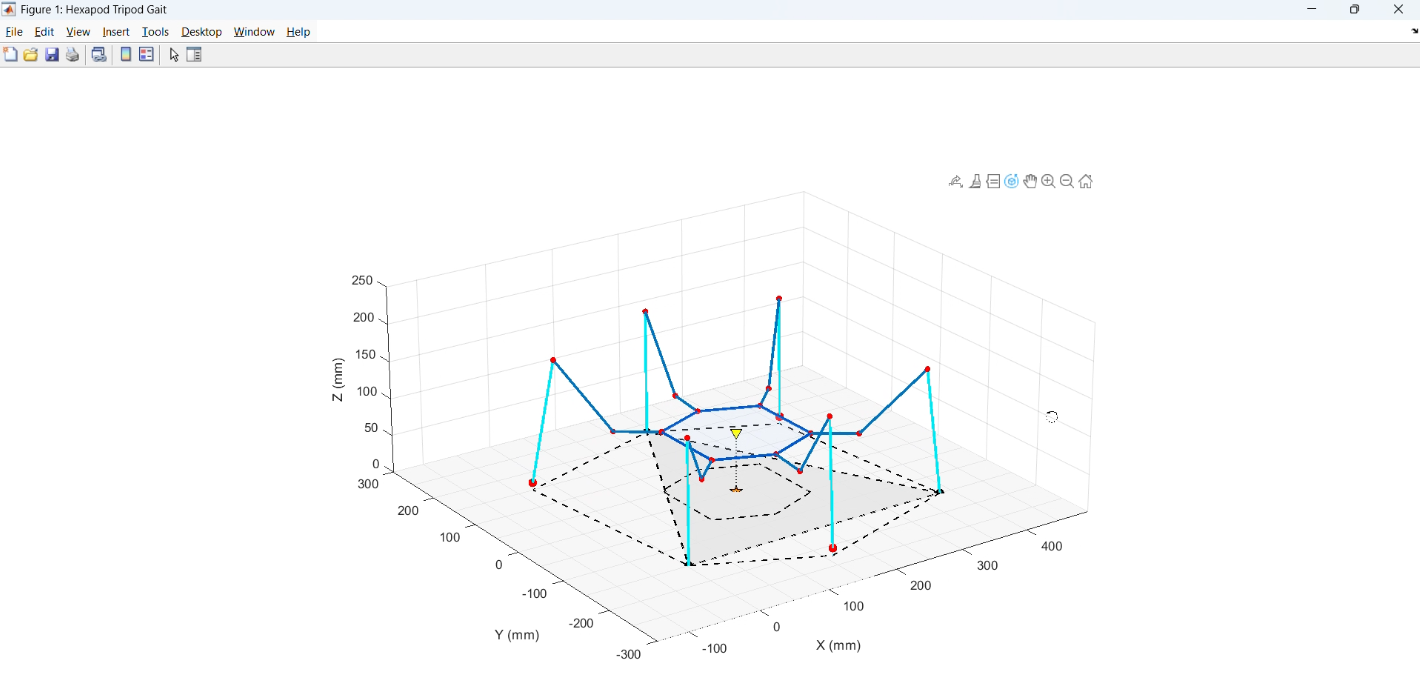
\includegraphics[width=0.85\textwidth]{pictures/MatlabResult.png}
    \caption{Kết quả mô phỏng chuyển động robot 6 chân trong MATLAB}
    \label{fig:matlab_result}
\end{figure}
 
 
% ============================================================
\section{Mô phỏng lực bằng phần mềm ANSYS}
% ============================================================
Trong đề tài này, ANSYS được sử dụng để mô phỏng khả năng chịu lực của kết cấu robot. Ngoài module Static Structural được áp dụng trực tiếp, phần mềm còn hỗ trợ các chức năng như: Coupled Field (mô phỏng bảng mạch điện tử, cảm biến siêu âm), Electric (phân tích điện trường, điện thế), Harmonic (mô phỏng dao động điều hòa), Hydrodynamic (tương tác kết cấu với môi trường nước) và LS-DYNA (động lực học phi tuyến tính).

\subsection{Thiết lập bài toán mô phỏng}
 
\subsubsection{Chọn vật liệu}
 
Vật liệu sử dụng chính trong thiết kế robot là nhựa in 3D PLA với các thông số:
 
\begin{table}[H]
    \centering
    \caption{Thông số vật liệu nhựa PLA}
    \label{tab:pla_material}
    \begin{tabular}{lll}
        \hline
        \textbf{Thông số} & \textbf{Giá trị} & \textbf{Đơn vị} \\
        \hline
        Khối lượng riêng & 1240 & kg/m$^3$ \\
        Mô đun đàn hồi & $3{,}5 \times 10^9$ & Pa \\
        Hệ số Poisson & 0{,}35 & -- \\
        Giới hạn chảy & 60 & MPa \\
        \hline
    \end{tabular}
\end{table}
 
\begin{figure}[H]
    \centering
    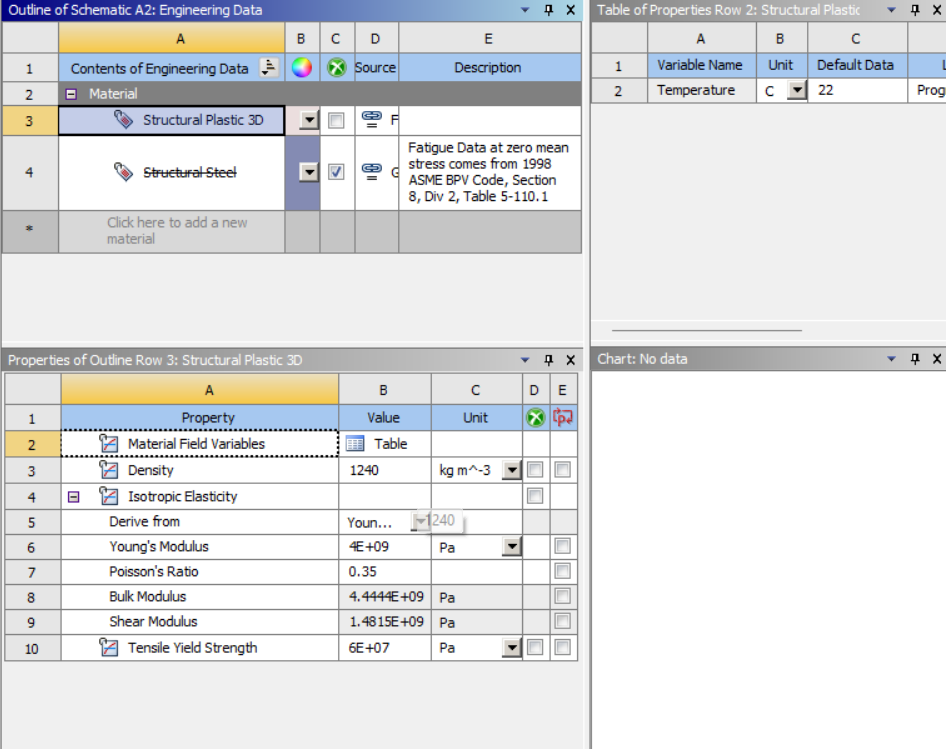
\includegraphics[width=0.75\textwidth]{pictures/AnsysMaterial.png}
    \caption{Gán vật liệu PLA cho mô hình trong ANSYS}
    \label{fig:ansys_material}
\end{figure}
 
\subsubsection{Nhập file bản vẽ mô phỏng}
 
ANSYS chỉ có thể đọc file dưới định dạng STEP và IGS. Do bản vẽ SolidWorks quá chi tiết sẽ gây khó khăn cho quá trình chia lưới phần tử, nên chỉ sử dụng bản vẽ đơn giản hóa để tiến hành mô phỏng chịu lực.
 
\begin{figure}[H]
    \centering
    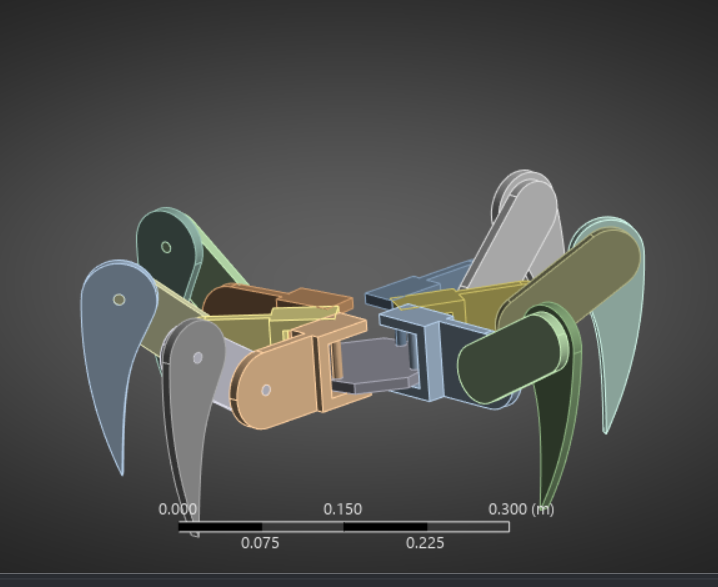
\includegraphics[width=0.75\textwidth]{pictures/AnsysImport.png}
    \caption{File bản vẽ đơn giản hóa được nhập vào ANSYS (định dạng STEP)}
    \label{fig:ansys_import}
\end{figure}
 
\subsubsection{Các bước tiến hành mô phỏng}
 
Quá trình mô phỏng chịu lực trong ANSYS được thực hiện theo các bước:
 
\begin{enumerate}
    \item Gán vật liệu cho từng phần tử của robot.
    \item Thiết lập các điểm liên kết (contact) giữa các chân, điểm nối và thân robot.
    \item Chia lưới phần tử (mesh); làm mịn lưới tại các vị trí chịu lực chủ đạo.
    \item Thêm điều kiện biên cố định tại các chân tiếp đất (trong thực tế, khi di chuyển chỉ có 3 chân chịu lực).
    \item Thêm tải trọng: trọng lực và tải bao gồm khối lượng các động cơ.
    \item Xuất các kết quả mong muốn (ứng suất, chuyển vị, biến dạng).
\end{enumerate}
 
\subsection{Kết quả mô phỏng}
 
\begin{figure}[H]
    \centering
    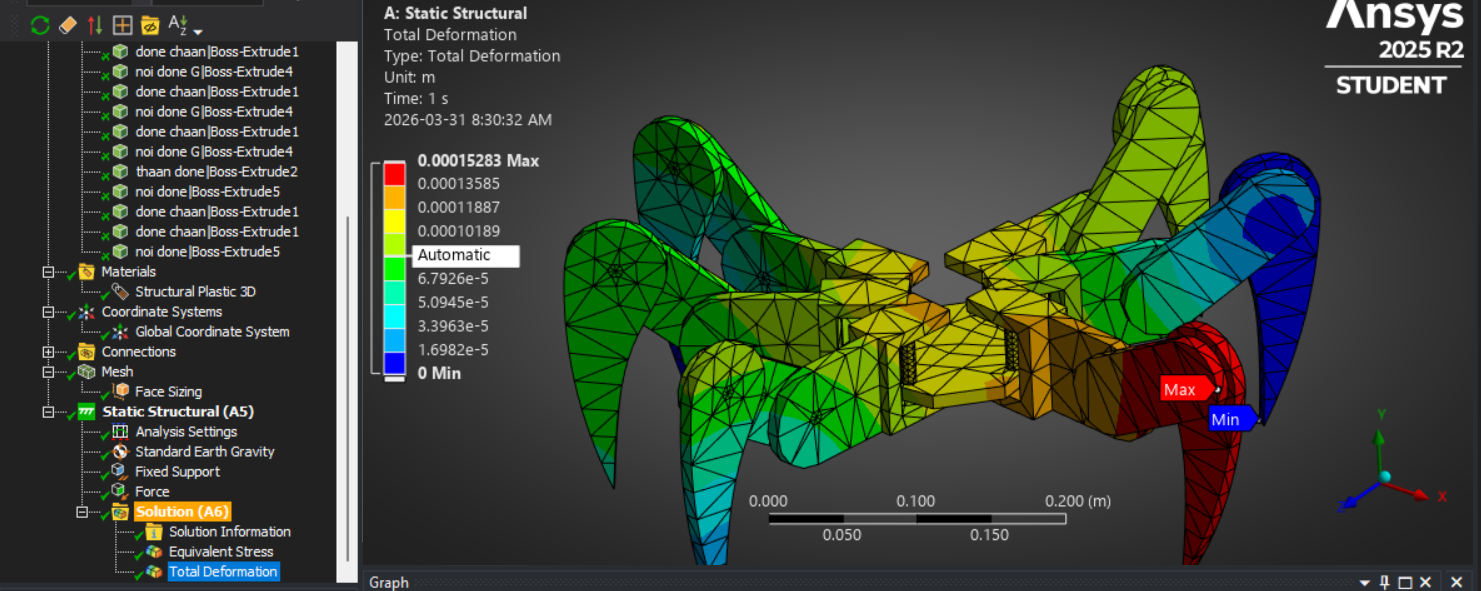
\includegraphics[width=0.9\textwidth]{pictures/AnsysResult.png}
    \caption{Kết quả phân tích lực trong ANSYS -- phân bố ứng suất và chuyển vị}
    \label{fig:ansys_result}
\end{figure}
 
\subsection{Nhận xét kết quả}
 
Kết quả mô phỏng cho thấy:
 
\begin{itemize}
    \item Biến dạng lớn nhất của kết cấu chỉ đạt \textbf{0{,}15 mm}, là giá trị rất nhỏ so với kích thước tổng thể của robot.
    \item Biến dạng theo phương ngang nhỏ hơn 2\% so với kích thước ngang, trong khi biến dạng theo phương đứng xấp xỉ 0\%.
    \item Các chân chịu lực khác nhau do góc tiếp đất khác nhau giữa các chân trong từng tư thế chuyển động.
\end{itemize}
 
Kết quả này khẳng định rằng kết cấu robot bằng nhựa PLA in 3D hoàn toàn đủ độ bền cơ học để hoạt động trong các điều kiện tải trọng thực tế của đề tài.
 
